\documentclass[conference]{IEEEtran}
% \usepackage{cite}
\usepackage{tikz, pgfplots}
\usepackage{amsmath,amssymb,amsfonts}
% \usepackage{algorithmic}
\usepackage{graphicx}
\usepackage{multirow}
% \usepackage{textcomp}
% \usepackage{xcolor}
\pgfplotsset{compat=1.18}
\graphicspath{{./images/}}
\def\BibTeX{{\rm B\kern-.05em{\sc i\kern-.025em b}\kern-.08em
    T\kern-.1667em\lower.7ex\hbox{E}\kern-.125emX}}

\begin{document}

\title{Differential Weight and Population Size of PRDE Traders: An Analysis of their Impact on Market Dynamics}

\author{\IEEEauthorblockN{George Herbert}
\IEEEauthorblockA{\textit{Department of Computer Science} \\
\textit{University of Bristol}\\
Bristol, United Kingdom \\
cj19328@bristol.ac.uk}
}

\maketitle

\begin{abstract}
This paper reports results from market experiments containing Paramaterized-Response Zero-Intelligence with Differential Evolution (PRDE) trader-agents.
Each PRDE trader-agent in a market simultaneously uses differential evolution (DE) to adapt their trading strategy to maximise profitability.
The DE algorithm within each PRDE trader is governed by two parameters: the differential weight coefficient $F$ and the number in population $\mathrm{NP}$.
Markets containing a homogeneous population of PRDE traders exhibit significantly different dynamics depending on the values of $F$ and $\mathrm{NP}$.
The first part of this paper explores the effect that $F$ and $\mathrm{NP}$ have on the profitability of markets populated by PRDE traders.
The latter part of this paper proposes a new algorithm based on PRDE to maximise profitability: the Parameterised-Response Zero-Intelligence with JADE (PRJADE) trader-agent.

\end{abstract}

\begin{IEEEkeywords}
Automated Trading, Financial Markets, Adaptive Trader-Agents, Differential Evolution
\end{IEEEkeywords}

\section{Introduction}

Adaptive automated trading algorithms have emerged as a transformative force in contemporary financial markets, enabling investors to harness the power of advanced computational techniques to gain a competitive edge in the marketplace.
Through the use of complex mathematical models and sophisticated algorithms, these cutting-edge technologies can analyse vast amounts of market data in real time, identifying and exploiting trading opportunities with speed and accuracy that were previously unimaginable.
As a result, the use of adaptive automated trading algorithms has become increasingly prevalent and has profoundly impacted how financial markets operate, shaping the fabric of the global economy.

However, these algorithms have generated much discussion and debate among experts, with some cautioning against their potential drawbacks.
For example, the `flash crash' in US financial markets on 6 May 2010, which saw the Dow Jones Industrial Average plummet almost 1,000 points in a matter of minutes, has been attributed partly to high-frequency trading algorithms aggressively reselling short-term positions to one another.
Despite these concerns, it is clear that these algorithms have become an inextricable part of the contemporary financial landscape, and their continued presence is all but guaranteed.
As such, researching these algorithms and their impact on contemporary markets is crucial for investors and researchers alike, to fully understand and navigate the rapidly evolving world of financial technology.

This report focuses on the \textit{Parameterised-Response Zero-Intelligence with Differential Evolution} (PRDE) trader-agent, which was recently introduced by Cliff in his research paper \cite{PRDE}.
The PRDE algorithm uses \textit{differential evolution} \cite{StornPrice} to continuously improve its trading strategy.
In his research, Cliff demonstrated that markets containing a homogeneous population of PRDE traders were more economically efficient overall than a baseline established when all traders used a simple stochastic hill-climbing strategy optimiser.

However, the PRDE traders implemented in Cliff's experiments did not vary in their parameter values.
This present study builds on Cliff's research by exploring the effects of altering the two critical parameters of the PRDE algorithm: the \textit{number in population} $\mathrm{NP}$ and the \textit{differential weight} $F$.
The $\mathrm{NP}$ parameter determines the number of strategies in a PRDE trader's private population, and the $F$ parameter determines the amount of perturbation applied to the strategies in the private population.

This present study examines the effects of changing these critical parameters on market dynamics using the \textit{Bristol Stock Exchange} (BSE) (see \cite{BSE, BSEPaper}), an open-source, high-fidelity simulation of an LOB-based financial exchange.
By analysing the effects of changing $F$ and $\mathrm{NP}$ on market behaviour, we can gain insights into how these algorithms influence market dynamics and how they can be optimised to maximise profitability.

\section{Background}

Gode and Sunder \cite{GodeSunder} revolutionised the field of experimental economics in 1993 with the advent of the \textit{Zero-Intelligence Constrained} (ZIC) trader-agent.
These agents, which generate quote prices uniformly at random from a predefined range, were shown to reproduce surprisingly human-like market dynamics.
In their original paper, Gode and Sunder defined the feasible range of trading prices as $[1,  200]$.
As such, a buyer with a limit price of $\lambda_B$ would generate quote prices from $\mathcal{U}(1, \lambda_B)$, whilst a seller with a limit price of $\lambda_S$ would generate quote prices from $\mathcal{U}(\lambda_S, 200)$.
Modern implementations of the ZIC model do not rely on a priori information about the feasible range, instead utilising the lowest and highest values in the order book as the bounds.
Cliff critiqued much of Gode and Sunder's work on ZIC in \cite{ZIP}, but the work that arose from the ZIC model is still widely used in studying market dynamics.
Many subsequent \textit{zero-intelligence} (ZI) and \textit{minimal-intelligence} (MI) trader-agents have stemmed from the work of Gode and Sunder.

One such ZI trader-agent, \textit{Parameterised-Response Zero-Intelligence} (PRZI) \cite{PRZI}, was recently introduced by Cliff.
PRZI is a nonadaptive generalisation of ZIC, in which the shape of the probability mass function (PMF) used to generate quote prices is governed by a strategy parameter $s\in[-1, 1]\in\mathbb{R}$.
This $s$-value determines the degree of `urgency' or `relaxation' in the trader's behaviour.
As $s\to1$, the distribution is evermore biased towards `urgent' quote prices---those closest to the least profitable price for the trader but most likely to attract a willing counterparty---conversely, as $s\to-1$, the distribution is biased towards `relaxed' quote prices---those that generate the most profit for the trader but are considerably less likely to attract a counterparty.
When $s=0$, the PMF is uniform, identical to that of a ZIC trader.

\textit{PRZI with Stochastic Hill-Climbing} (PRSH) \cite{PRSH} is an adaptive extension to PRZI, also introduced by Cliff.
The algorithm dynamically alters the strategy parameter $s$ in an attempt to increase profitability.
A given PRSH trader $i$ maintains a private local population $\mathcal{S}_i$ of $k$ strategy parameters, each of which it evaluates via a loop to identify the most profitable.
The most profitable strategy is `mutated' via a stochastic mutation function to produce $k-1$ mutants, and this set of $k$ strategies constitutes the new $\mathcal{S}_i$.

\textit{PRZI with Differential Evolution} (PRDE) \cite{PRDE} is the latest adaptive extension to PRZI introduced by Cliff.
It replaces the simple stochastic hill-climber in PRSH with a DE optimisation system \cite{StornPrice}.
A given PRDE trader $i$ maintains its own DE system with a population of candidate $s$-values $\mathcal{S}_i$ of size $\mathrm{NP}\ge4$ denoted by $s_{i,1},s_{i,2},...,s_{i,\mathrm{NP}}$.
Once trader $i$ has evaluated a particular strategy $s_{i,x}$, three other distinct $s$-value are chosen at random: $s_{i,r_1}$, $s_{i,r_2}$ and $s_{i,r_3}$ such that $x\ne r_1\ne r_2\ne r_3$.
A new candidate strategy $s_{i,y}$ is constructed as follows:
\[
s_{i,y}\leftarrow\max(\min(s_{i,r_1}+F_i(s_{i,r_2}-s_{i,r_3}),1), -1)
\]
where $F_i$ is trader $i$'s differential weight coefficient.
The fitness of $s_{i,y}$ is evaluated, and if it performs better than $s_{i,x}$ then $s_{i,y}$ replaces $s_{i,x}$; otherwise, it is discarded and the next randomly selected strategy is evaluated.
PRDE also includes a `mega-mutation' mechanism to deal with convergence issues that arise from $s_{i,r_2}-s_{i,r_3}$ tending very close to zero in a highly-converged population.
Suppose at any time the standard deviation of the candidate $s$-values in trader $i$'s private population is less than $0.0001$.
In that case, a randomly selected candidate $s_{i,r}$ is given a value sampled randomly from $\mathcal{U}(-1,1)$.

\section{Homogeneous Exploration of $F$ and $\mathrm{NP}$}

\subsection{Overview of the Combined Effect of $F$ and $\mathrm{NP}$}

According to Cliff's research in \cite{PRDE}, using DE as the adaption mechanism for each trading entity in a market can double the profit extracted through traders' interactions, compared to using a stochastic hill-climber as the adaption mechanism.
However, in his simulations, Cliff only experimented with $F=0.8$ and $\mathrm{NP}=4$ for the PRDE traders.
As such, the initial experiments in this paper serve as a follow-up: to analyse the combined effect that different values of $F$ and $\mathrm{NP}$ have on profitability.
I designed a set of experiments with a similar setup as Cliff, in which BSE was used to simulate a financial market for a single abstract tradeable commodity.
In each market simulation, I implemented a homogeneous population of $N_T=30$ PRDE traders with an equal number of buyers $N_B$ and sellers $N_S$ (i.e. $N_B=N_S=15$).
The population in a given experiment was homogeneous with respect to the fact that all PRDE traders had the same differential weight $F$ and the same number in population $\mathrm{NP}$.
Each simulation had what economists call perfect elasticity of supply and demand.
All $N_B$ buyers were provided with a limit price of $\lambda_B=\$140$ per unit, while all $N_S$ sellers were provided with a limit price of $\lambda_S=\$60$ per unit.
This supply and demand schedule produces a market in which every active trader could, in theory, find a willing counterparty to trade.
In the simulation, after two traders engaged in a trade, they were rendered inactive until their stock was replenished, which occurred approximately every five seconds.
I ran each experiment for 100 simulated days on an Apple MacBook Pro with the M1 Pro chip, which took approximately three hours running at 800x real-time.

Figure \ref{profit_grid} displays a heatmap showing the combined profit extracted from the market by the population of $N_B$ buyers and $N_S$ sellers.
Since each experiment used an identical quantity of traders and limit prices, the theoretical maximum profit that could have been extracted from each experiment was also identical.
As such, the actual total profit extracted is indicative of market efficiency.
There is a clear association between the configuration of $F$ and $\mathrm{NP}$ and the efficiency of the market.
Namely, large values of $F$ combined with moderately large values of $\mathrm{NP}$ produce the most efficient market.
$F=2$ and $\mathrm{NP}=14$ produced the most efficient market; 3.75\% more profit was extracted than the $F=0.8$ and $\mathrm{NP}=4$ configuration that Cliff used \cite{PRDE}.

\begin{figure}[htbp]
    \centerline{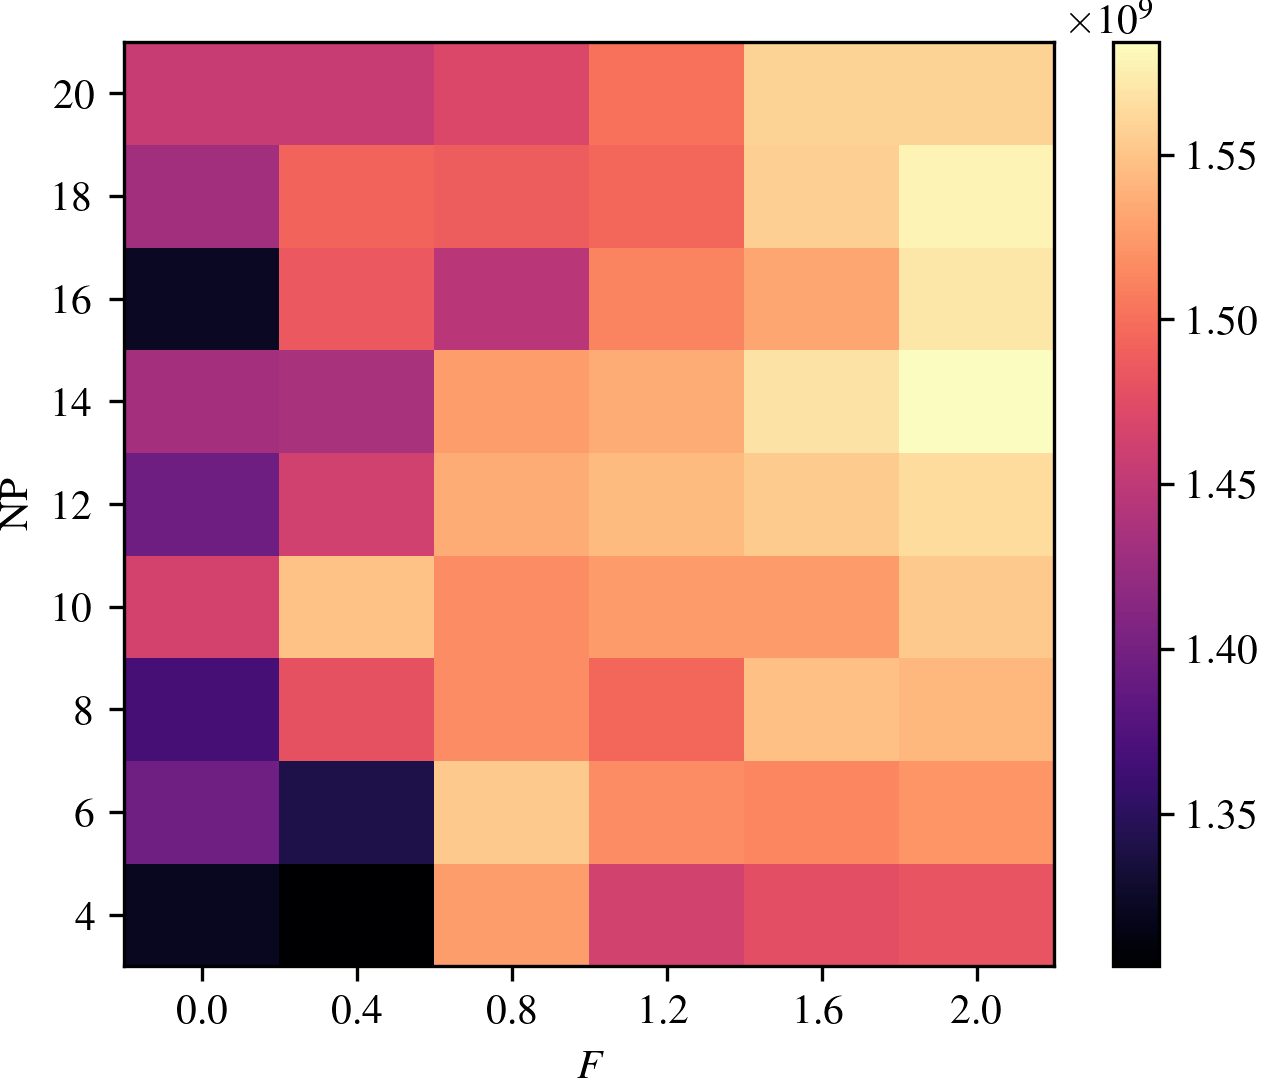
\includegraphics[width=\columnwidth]{profit_grid.png}}
    \caption{
        Relationship between different combinations of $F$ and $\mathrm{NP}$, and the total profit extracted by all PRDE traders in the market.
        The horizontal axis is $F$; the vertical axis is $\mathrm{NP}$.
        The intensity of pixel shading represents the total profit extracted from the market during a single 100-day simulation.
        See text for further discussion.
    }
    \label{profit_grid}
\end{figure}

Much of the relationship can be attributed to $F$ and $\mathrm{NP}$'s influence over the `urgency' of the traders.
There is a moderately strong positive correlation with $R^2=0.72$ between the total amount of time the traders in the market spent playing `very urgent' strategies (i.e. $s>0.5$) and the total profit extracted from the market, as evident in Figure \ref{strategy_profit}.

\begin{figure}[htbp]
    \centerline{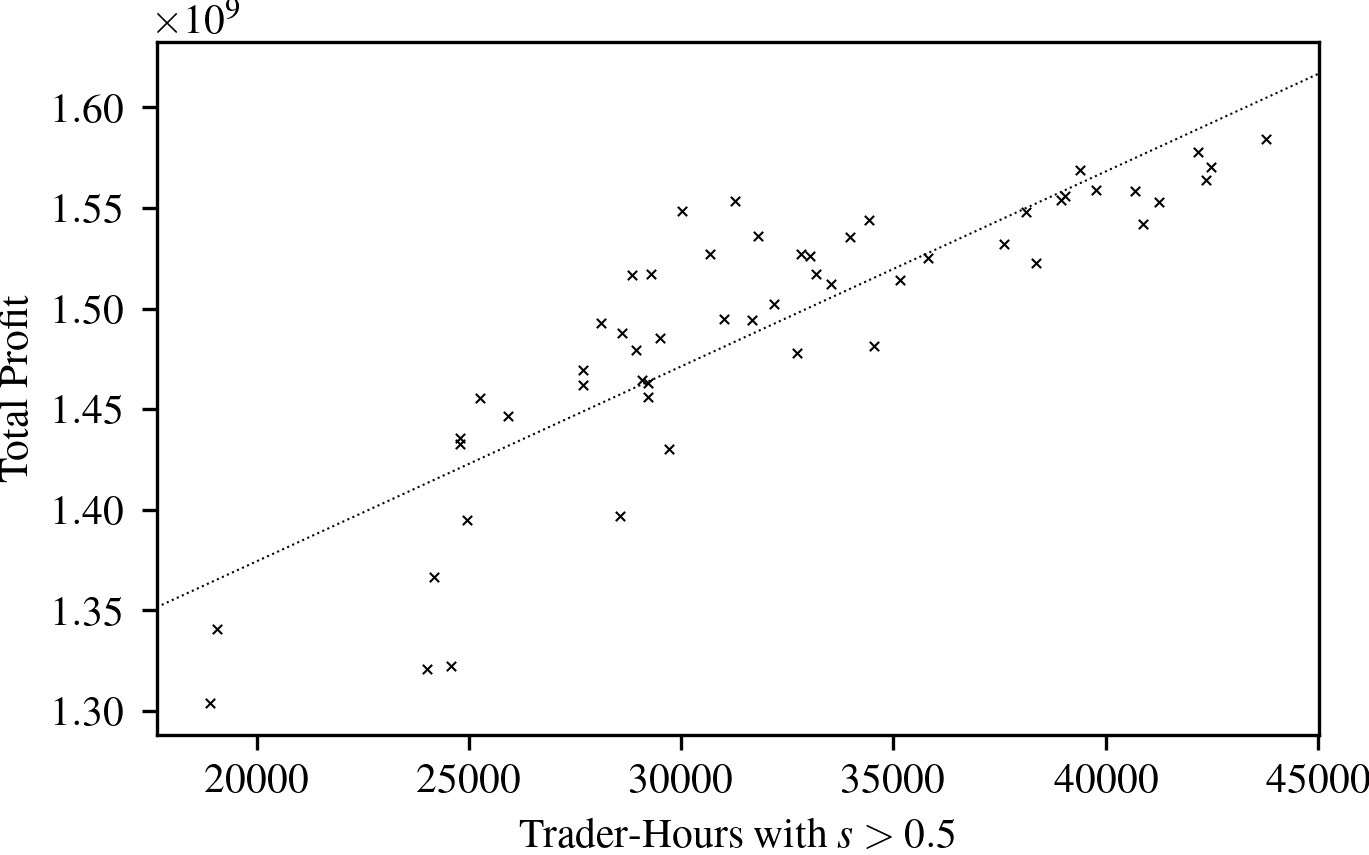
\includegraphics[width=\columnwidth]{strategy_profit.png}}
    \caption{
        Relationship between the amount of time traders spent playing $s$-values greater than 0.5 and the total profit extracted by all traders in the market.
        The line shows linear regression; $R^2=0.72$.
        The horizontal axis is the cumulative number of hours traders spent playing $s$-values where $s>0.5$; the vertical axis is the total profit extracted from the market during a given 100-day simulation.
        See text for further discussion.
    }
    \label{strategy_profit}
\end{figure}

To understand this relationship, one must consider how the $s$-value of a given PRDE trader at a particular point in time affects the probability of it finding a counterparty to trade.
For a given trader, as $s\to1$ (i.e. increasingly `urgent'), the trader's quote prices are evermore likely to attract a counterparty; the reverse is true as $s\to-1$ (i.e. increasingly `relaxed').
Therefore, a strong relationship exists between the amount of time the traders in the market are `urgent' and the number of trades.
Due to each experiment having perfect elasticity of supply and demand, for a given trade at price $P$, the seller's profit can be denoted $P-\lambda_S$, whilst the buyer's profit can be denoted $\lambda_B-P$.
Therefore, the combined profit is as follows:
\[
  (P-\lambda_S) + (\lambda_B-P)=\lambda_B-\lambda_S
\]
In other words, the profit extracted from the market from any given trade is constant.
As such, the total profit extracted in a given 100-day market session is directly proportional to the number of trades, which, as mentioned, is related to the amount of time traders in the market are `urgent'.

\subsection{Analysis of the Effect of $F$}

As mentioned, a significant amount of the variance in the efficiency of the market can be explained by the amount of time the traders spend playing $s$-values greater than 0.5.
To this end, the the differential weight's influence on the total profitability can be primarily attributed to how it influences the `urgency' of the traders.
The market simulation data showed a moderately strong positive correlation with $R^2=0.77$ between $F$ and the amount of time the traders spent playing $s$-values greater than 0.5, as shown in Figure \ref{F_strats}.

\begin{figure}[htbp]
    \centerline{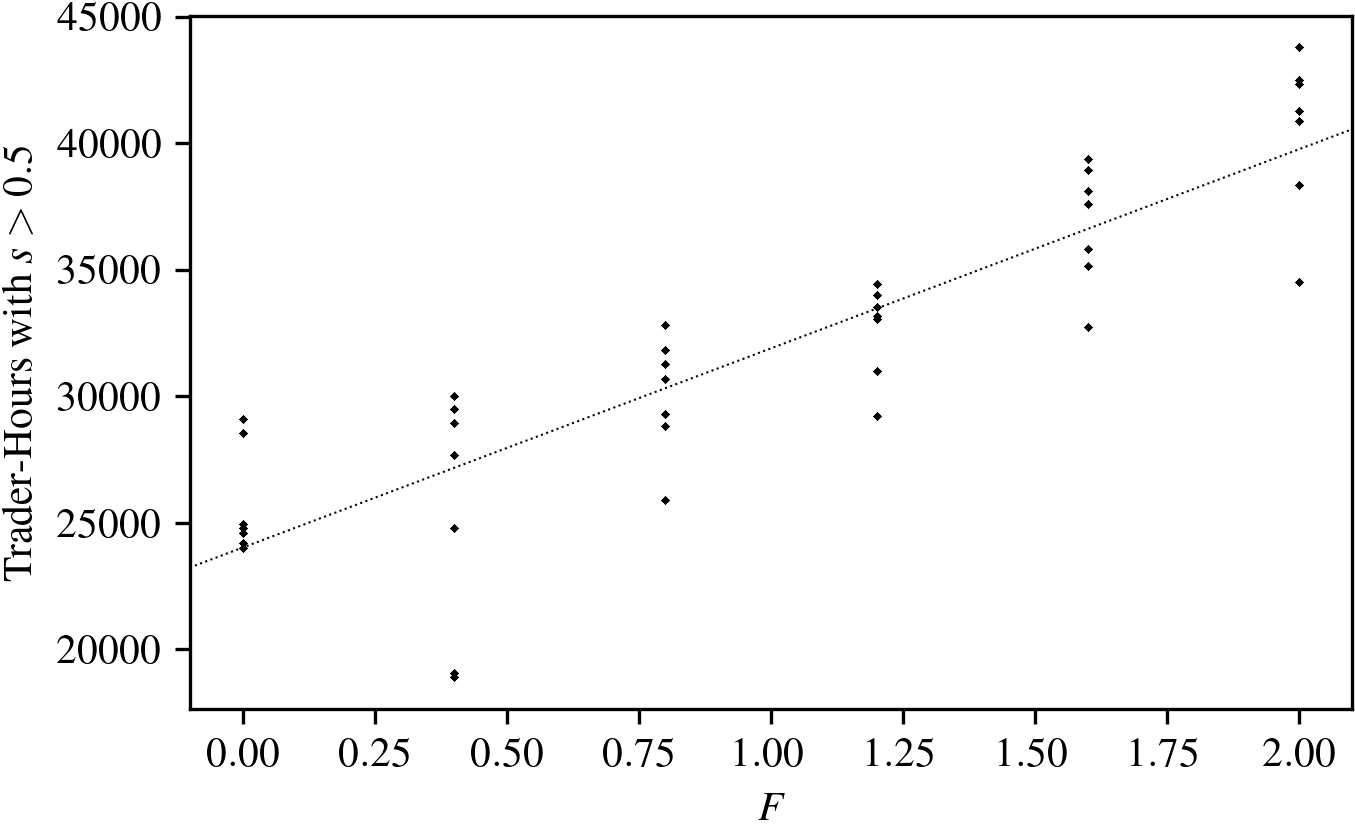
\includegraphics[width=\columnwidth]{F_strats.png}}
    \caption{
        Relationship between $F$ and the amount of time traders spent playing $s$-values greater than 0.5
        The line shows linear regression; $R^2=0.77$.
        The horizontal axis is the differential weight coefficient $F$; the vertical axis is the number of trader-hours where $s>0.5$.
        See text for further discussion.
    }
    \label{F_strats}
\end{figure}

This relationship manifests due to $F$'s impact on the `urgency' of the PRDE traders throughout the market session.
For larger values of $F$, the proportion of traders playing with $s>0.5$ increases significantly faster.
Figure \ref{k=14_strats} shows an example of this when $\mathrm{NP}=14$.
When $F=2$, the proportion of traders trading with $s>0.5$ increased quickly: the seven-day moving average of the percentage of traders playing $s$-values that were $s>0.5$ rose to over 60\% after just 40 days.
Conversely, when $F=0.8$, the moving average was only approximately 45\% after the same amount of time.

\begin{figure}[htbp]
    \centerline{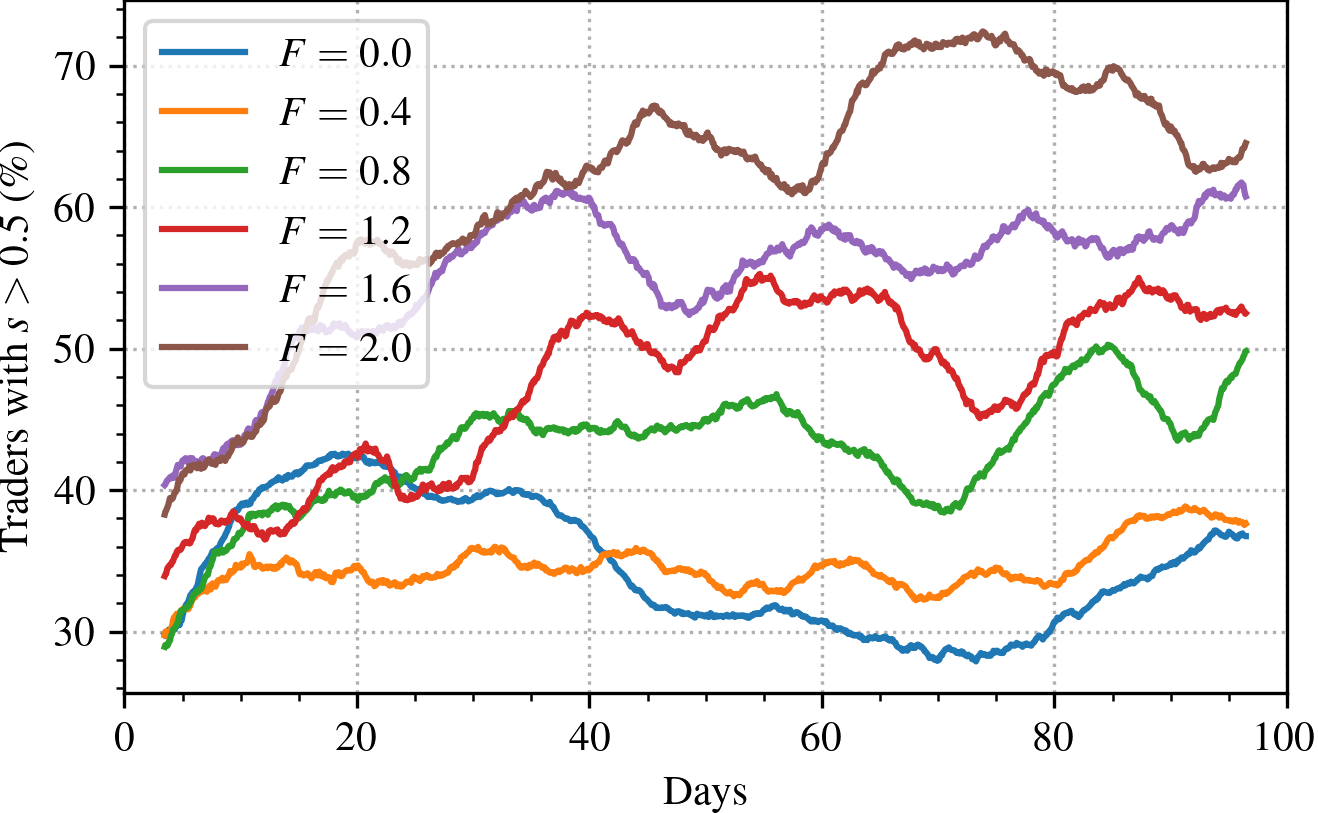
\includegraphics[width=\columnwidth]{k=14_strats.png}}
    \caption{
        Plot of the percentage of traders playing $s$-values of $s>0.5$ from multiple 100-day experiments in a market populated entirely by PRDE traders.
        The horizontal axis is time, measured in days; the vertical axis is the proportion of traders with an $s$-value of $s>0.5$.
        Each line is a seven-day simple moving average of the percentage for different values of $F$ when $\mathrm{NP}=14$.
        See text for further discussion.
    }
    \label{k=14_strats}
\end{figure}

The reason for this effect can be explained mathematically.
Taking the extreme example of $F_i=0$ for trader $i$, the equation to derive a new candidate strategy $s_{i,y}$ to replace $s_{i,x}$ becomes $s_{i,y}\leftarrow s_{i,r_1}$.
Therefore, following the evaluation period of $s_{i,y}$, the value of $s_{i,x}$ can either remain the same or take on the value of $s_{i,r_1}$, in which case two or more of the $s$-values in the local population $\mathcal{S}_i$ will be identical---the `genetic diversity' will be reduced.
The only time a new $s$-value can be introduced into $\mathcal{S}_i$ is when the diversity of $s$-values becomes so constrained that a `mega-mutation' occurs, in which case the algorithm samples a new $s$-value from $\mathcal{U}(-1,1)$.
As a result, the distribution of $s$-values in the entire population of PRDE traders struggles to deviate significantly from uniformity throughout the 100-day market session.
This uniformity ultimately produces a market containing a wide range of both `urgent' and `relaxed' buyers and sellers, which is inefficient since many of the more `relaxed' traders will be unable to find a willing counterparty.
An example of such a distribution of $s$-values can be seen in Figure \ref{k=14,F=0.0_buy_strats}, which displays a heatmap of individual strategy values for the proportion of 15 PRDE buyers when $F=0$ and $\mathrm{NP}=14$.
While the case of $F=0$ is extreme, I found experimentally that the market increasingly exhibits the inefficient dynamics described here as $F$ tends towards $0$.

\begin{figure}[htbp]
    \centerline{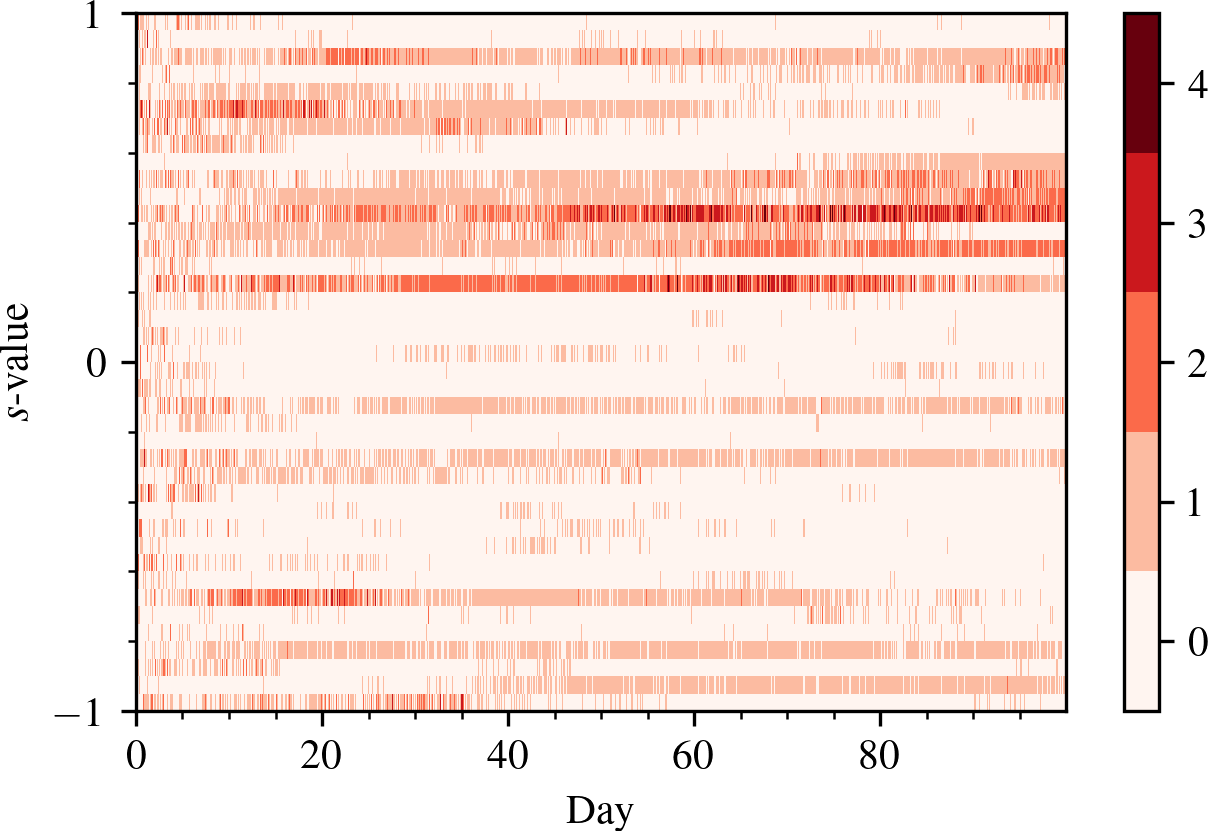
\includegraphics[width=\columnwidth]{k=14,F=0.0_buy_strats.png}}
    \caption{
        Heatmap of individual $s$-values for the population of 15 PRDE buyers in a market populated entirely by PRDE traders with $F=0$ and $\mathrm{NP}=14$.
        The horizontal axis is time, measured in days; the vertical axis is the $s$-value pixelated into 40 bins of size 0.05.
        The intensity of pixel shading increases with the number of PRDE buyers in the population currently trading with an $s$-value in the 0.05 range.
        See text for further discussion.
    }
    \label{k=14,F=0.0_buy_strats}
\end{figure}

On the other extreme of the spectrum, when $F=2$, a very different market dynamic tends to manifest.
This dynamic difference is evident in Figure \ref{k=14,F=2.0_buy_strats}, which displays a heatmap for the 15 PRDE buyers with $F=2$ and $\mathrm{NP}=14$.
Unlike the more uniform distribution of $s$-values exhibited when $F=0$, the $s$-values in Figure \ref{k=14,F=2.0_buy_strats} were bimodal at the two extremes of $s\approx-1$ and $s\approx1$, with the peak at $s=1$ slightly more prominent.
Moreso, both the buyers and sellers displayed this behaviour.
Again, this can be explained mathematically using the equation to derive a new candidate strategy $s_{i,y}$ to replace $s_{i,x}$.
The value of the differential weight $F_i$ is directly proportional to $F_i(s_{i,r_2}-s_{i,r_3})$.
Thus, assuming $s_{i,r_2}-s_{i,r_3}$ is non-zero, the value of $s_{i,y}$ is more likely to be $-1$ or $1$ as $F_i$ increases.
This bimodal distribution induces a market dynamic in which there are very quickly many extremely `urgent' and extremely `relaxed' buyers and sellers.
It is this large number of urgent traders that exist throughout the market session that enables a large amount of profit to be extracted from the market.
Furthermore, I found experimentally that this bimodal behaviour is ever more prominent for larger values of $F$.

\begin{figure}[htbp]
    \centerline{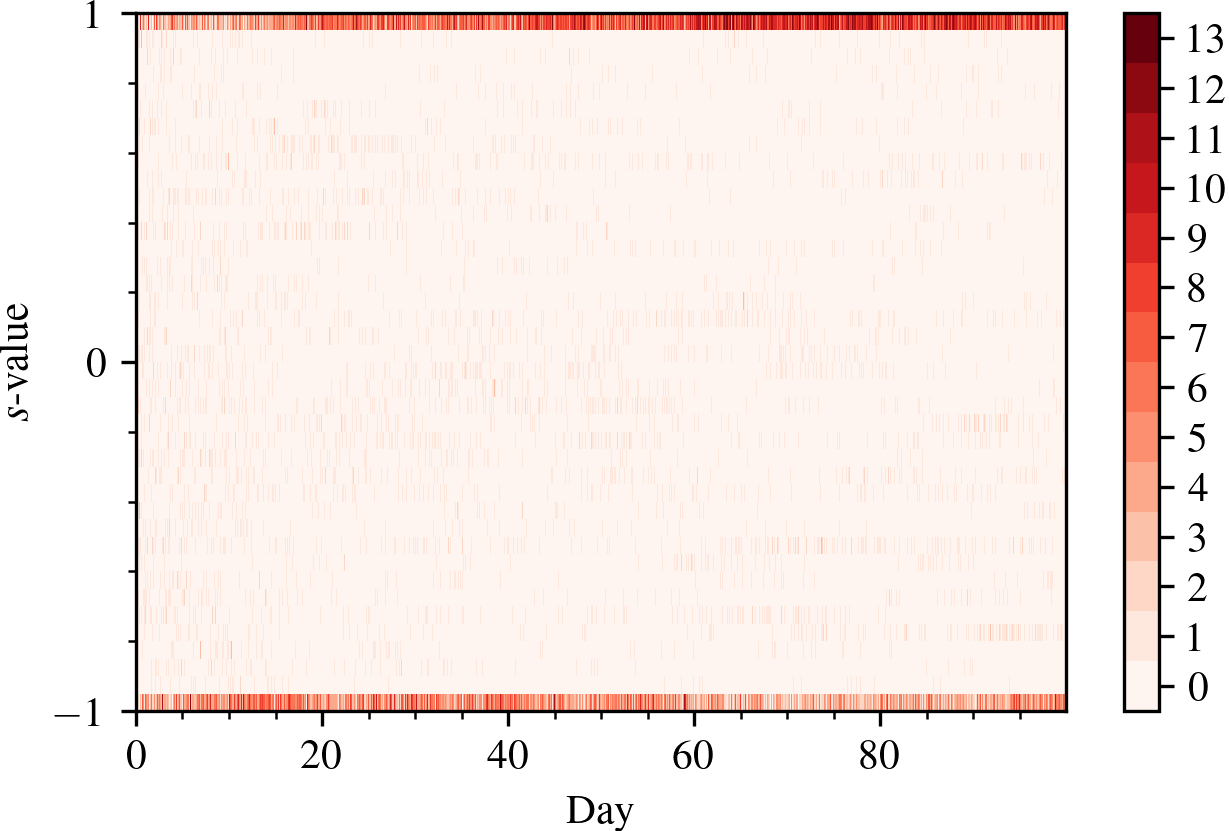
\includegraphics[width=\columnwidth]{k=14,F=2.0_buy_strats.png}}
    \caption{
        Heatmap of individual $s$-values for the population of 15 PRDE buyers in a market populated entirely by PRDE traders with $F=2$ and $\mathrm{NP}=14$.
        The format is the same as in Figure \ref{k=14,F=0.0_buy_strats}.
        See text for further discussion.
    }
    \label{k=14,F=2.0_buy_strats}
\end{figure}

\subsection{Analaysis of the Effect of $\mathrm{NP}$}

The effect of the number in population on the market's efficiency is similarly primarily driven by its influence over the `urgency' of the traders.
However, unlike the relationship with the differential weight, the relationship between $\mathrm{NP}$ and the amount of time traders spend playing $s$-values greater than 0.5 cannot be modelled linearly.
The data from the market simulations showed that the relationship is highly dependent on the value of $F$.
For smaller values of $F$, the influence of $\mathrm{NP}$ is significantly noisy, as shown in Figure \ref{profit_grid}.
However, for larger values of $F$, the relationship can best be modelled using a quadratic curve, as shown in Figure  \ref{F=2.0_strats}.
The quadratic demonstrates that the association between $\mathrm{NP}$ and the `urgency' of traders is more complex and dynamic than a simple linear model can capture.

\begin{figure}[htbp]
    \centerline{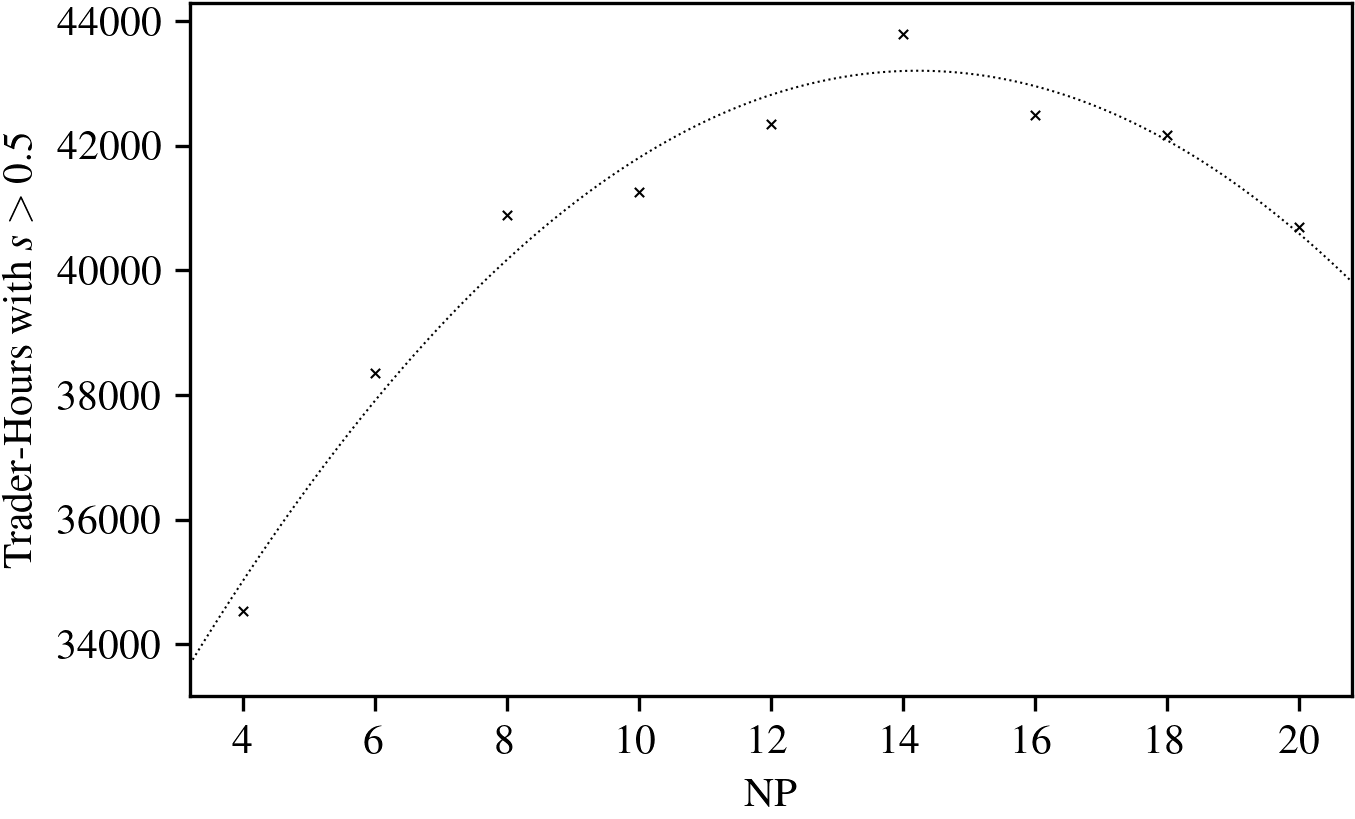
\includegraphics[width=\columnwidth]{f=2.0_strats.png}}
    \caption{
        Relationship between $\mathrm{NP}$ and the number of trader-hours in the market playing `very urgent' $s$ values greater than 0.5 when $F=2.0$.
        The line shows quadratic regression; $R^2=0.96$.
        The horizontal axis is the number in population $\mathrm{NP}$; the vertical axis is the number of trader-hours where $s>0.5$.
        See text for further discussion.
    }
    \label{F=2.0_strats}
\end{figure}

This quadratic relationship can be explained as the combined effect of two influencing factors.
The first influencing factor comes from $\mathrm{NP}$'s effect on the number of $s$-values greater than 0.5 that a given PRDE trader $i$ can sustain in its private population $\mathcal{S}_i$.
The second influencing factor comes from $\mathrm{NP}$'s effect on the time it takes the traders in the market to improve on the initial random conditions.

As mentioned, larger values of $F$ induce a bimodal distribution of $s$-values at $s\approx -1$ and $s\approx 1$.
Using $\mathrm{NP}=\mathrm{4}$ as an example, an individual trader can have at most three $s$-values of $s\approx 1$, because as soon as the fourth $s$-value becomes 1, a `mega-mutation' occurs---this equates to a maximum of only 75\% of the $s$-values in their private population $\mathcal{S}_i$ at $s\approx 1$.
Conversely, when $\mathrm{NP}$ is larger, individual traders can accumulate a more significant proportion of $s$-values of $s\approx 1$ in their private populations without a `mega-mutation'.
The ability to accumulate a more significant proportion means that homogeneous populations of PRDE traders with larger values of $\mathrm{NP}$ produce a market dynamic with more `very urgent' traders, which produces a more efficient market.
The effect of $\mathrm{NP}$ is noiser for smaller values of $F$ for the same reason.
As mentioned, the bimodal distribution is ever less prevalent with smaller values of $F$, so the impact of $\mathrm{NP}$ is less relevant as the `mega-mutations' do not occur as often, regardless.

The primary reason this trend is nonlinear is that for large values of $\mathrm{NP}$, an inverse relationship between $\mathrm{NP}$ and the number of `very urgent' traders in the market manifests.
The inverse relationship is because, for a given PRDE trader, the probability that an $s$-value in the trader's private population is selected to be evaluated next is $\mathrm{NP}^{-1}$.
Therefore, in homogeneous populations of PRDE traders with larger values of $\mathrm{NP}$, it takes significantly longer to iteratively improve on the initial random conditions in the entire local population of $s$-values.
As a result, it takes significantly longer for the PRDE traders to accumulate a large number of $s$-values greater than 0.5, meaning the market is less efficient.
On the furthest end of the spectrum, as $\mathrm{NP}\to\infty$, the PRDE traders in the market would be completely unable to improve on the initial random conditions of the market.

\section{PRDE in a Heterogeneous Market}

The experiments conducted in the previous section were designed to build on the work in \cite{PRDE}.
By using different combinations of $F$ and $\mathrm{NP}$ in each experiment, I was able to study the impact of these parameters on market efficiency.
The results showed that the most profitable combination of $F$ and $\mathrm{NP}$ was 22\% more profitable than the least profitable.

However, the experimental setup was simplistic: the markets were homogeneously populated and had perfect elasticity of supply and demand.
While this provided highly interpretable results and an important insight into the influence of $F$ and $\mathrm{NP}$ on a homogeneous coevolutionary metapopulation of PRDE traders, it did not accurately represent most contemporary financial markets.
Most markets contain a population of distinct adaptive automated trading algorithms and do not have perfect elasticity of supply and demand.
As such, I conducted a series of follow-up experiments that better represented these contemporary markets. 
The primary purpose of the follow-up experiments was to identify any tangible association between the performance of each combination of $F$ and $\mathrm{NP}$ in the two sets of experiments.
By doing so, I sought to identify whether a definitive `optimal' combination existed that would consistently provide maximum profitability, regardless of the market.

In each market simulation on BSE, I implemented a population of $N_T=20$ traders with an equal number of buyers $N_B$ and sellers $N_S$ (i.e. $N_B=N_S=10$).
In order to introduce a form of heterogeneity into the market, each of the $N_B$ buyers and $N_S$ sellers were comprised of five PRDE trader-agents and five Zero-Intelligence Plus (ZIP) \cite{ZIP} trader-agents.
ZIP is a widely-studied MI agent that employs an elementary form of machine learning and was one of the first trader-agents demonstrated to perform better than humans \cite{DasHansonKephartTesauro}.
All PRDE traders in a given experiment had identical values of $F$ and $\mathrm{NP}$.
To better represent contemporary financial markets' supply and demand curves, the $N_B$ buyers and $N_S$ sellers were provided distinct, evenly-spaced limit prices in the range $[60, 140]$.
In the simulation, after two traders engaged in a trade, they were rendered inactive until their stock was replenished, which occurred approximately every five simulated seconds.
I ran each experiment for 100 simulated days.

Figure \ref{zip_profit_grid} displays a heatmap showing the combined profit extracted from the market by the population of 10 PRDE traders from each experiment.
The difference in profitability for different combinations of $F$ and $\mathrm{NP}$ was significant: the most profitable combination of $F$ and $\mathrm{NP}$ extracted 322\% more profit on average than the least profitable combination.
While some of this effect is likely due to stochasticity inherent in market simulations, it suggests that one would require a priori information about the market to deploy a PRDE trader with a near-optimal choice of $F$ and $\mathrm{NP}$.

\begin{figure}[htbp]
    \centerline{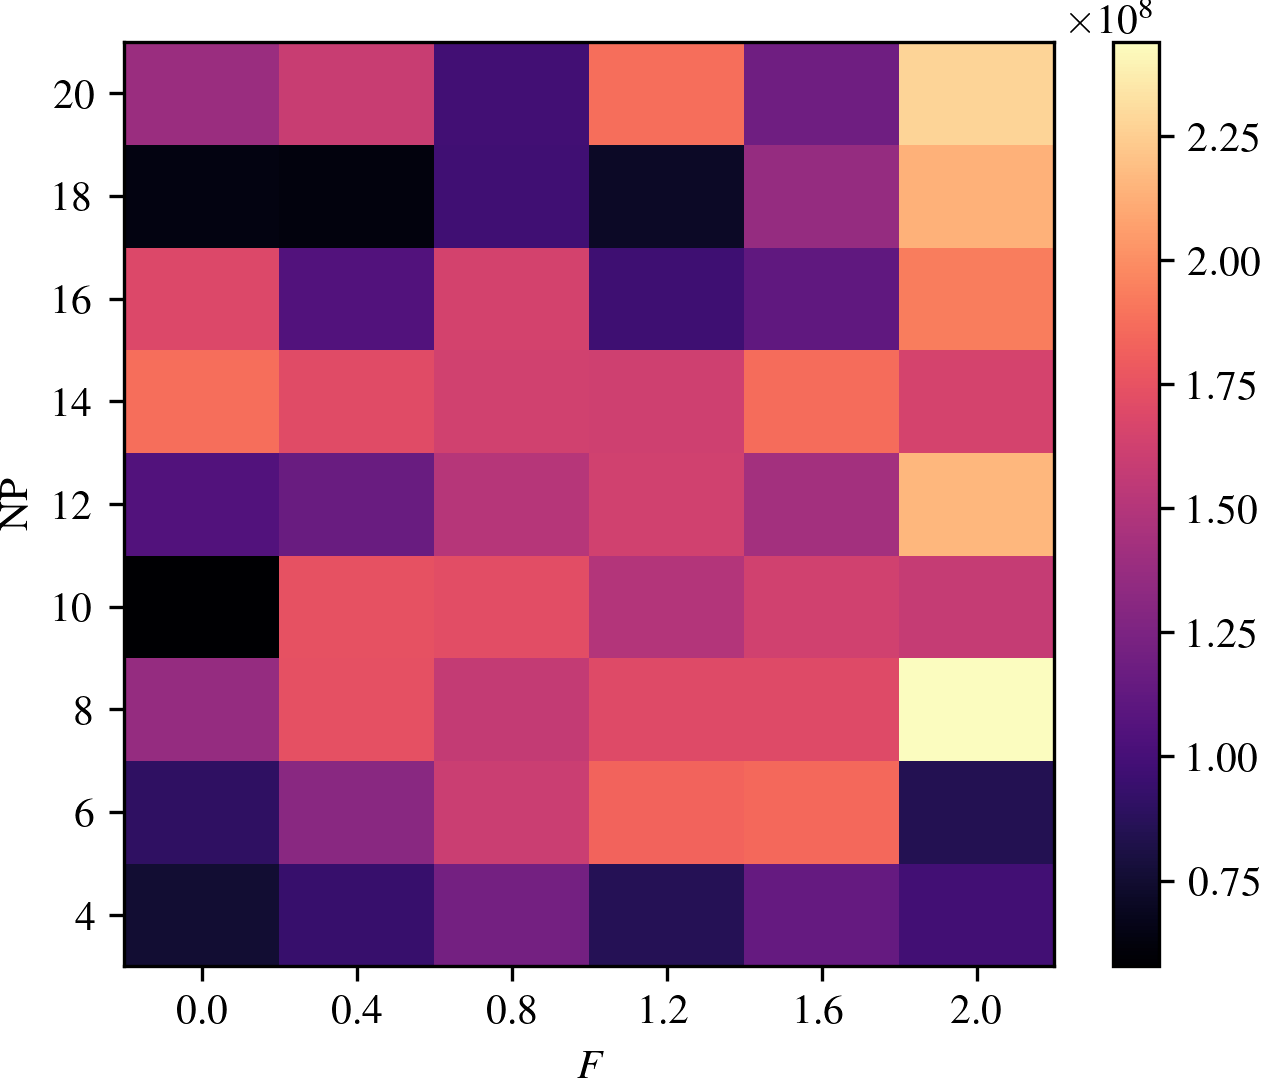
\includegraphics[width=\columnwidth]{zip_profit_grid.png}}
    \caption{
        Relationship between the differential weight coefficient $F$, the number in population $\mathrm{NP}$ and the total profit extracted by all PRDE traders in the market.
        The format is the same as in Figure \ref{profit_grid}.
        See text for further discussion.
    }
    \label{zip_profit_grid}
\end{figure}

Several loose similarities can be observed with the heatmap from the previous set of experiments in Figure \ref{profit_grid}.
However, there is no discernible statistically significant relationship between the profitability of a PRDE trader with a given combination of $F$ and $\mathrm{NP}$ in the homogeneous experiments and the same combination in the heterogeneous experiments, as evident in Figure \ref{homo_zip_scatter}.
The lack of association indicates that the effect of $F$ and $\mathrm{NP}$ is highly dependent on either traders' behaviour, the supply and demand schedules, or, most likely, a combination of both.

It is evident that the heterogeneous markets with stepped supply and demand schedules clearly exhibit different behaviours from Figure \ref{ZIP_strategy_profit}.
Unlike in the homogeneous experiments with perfect elasticity of supply and demand, there is no longer a linear relationship between the total time the PRDE traders in the market spent playing `very urgent' strategies (i.e. $s>0.5$) and the total profit extracted by them.
As such, though larger $F$ values still induce a more bimodal distribution of $s$-values, the relationship between $F$ and the total profit extracted is not the same.

\begin{figure}[htbp]
    \centerline{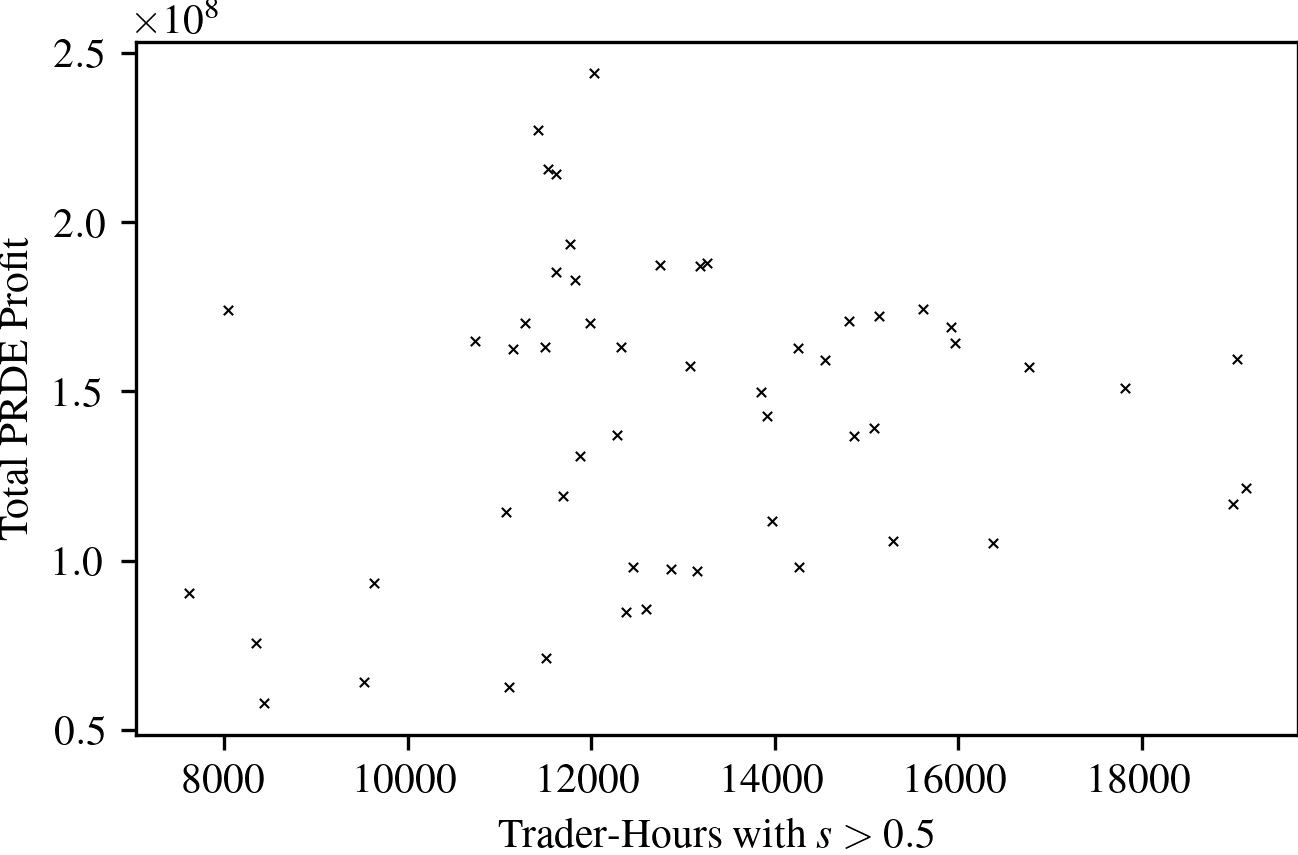
\includegraphics[width=\columnwidth]{ZIP_strategy_profit.png}}
    \caption{
        Relationship between the amount of time traders spent playing $s$-values greater than 0.5 and the total profit extracted by all traders in the market by the PRDE traders in the heterogeneous experiments.
        The format is the same as in Figure \ref{strategy_profit}
        See text for further discussion.
    }
    \label{ZIP_strategy_profit}
\end{figure}

Profitability being dependent on certain conditions is a common theme in the broader literature on adaptive autonomous trader-agents.
The `dominance' of any given algorithm is often contingent on the other trader-agents in the market (e.g. \cite{Vach}).
Therefore, while there are clear values of $F$ and $\mathrm{NP}$ that produce consistently poor results, namely $F=0$, I cannot conclusively say that there exists any single `optimal' combination that will consistently extract the maximum profit.

\begin{figure}[htbp]
    \centerline{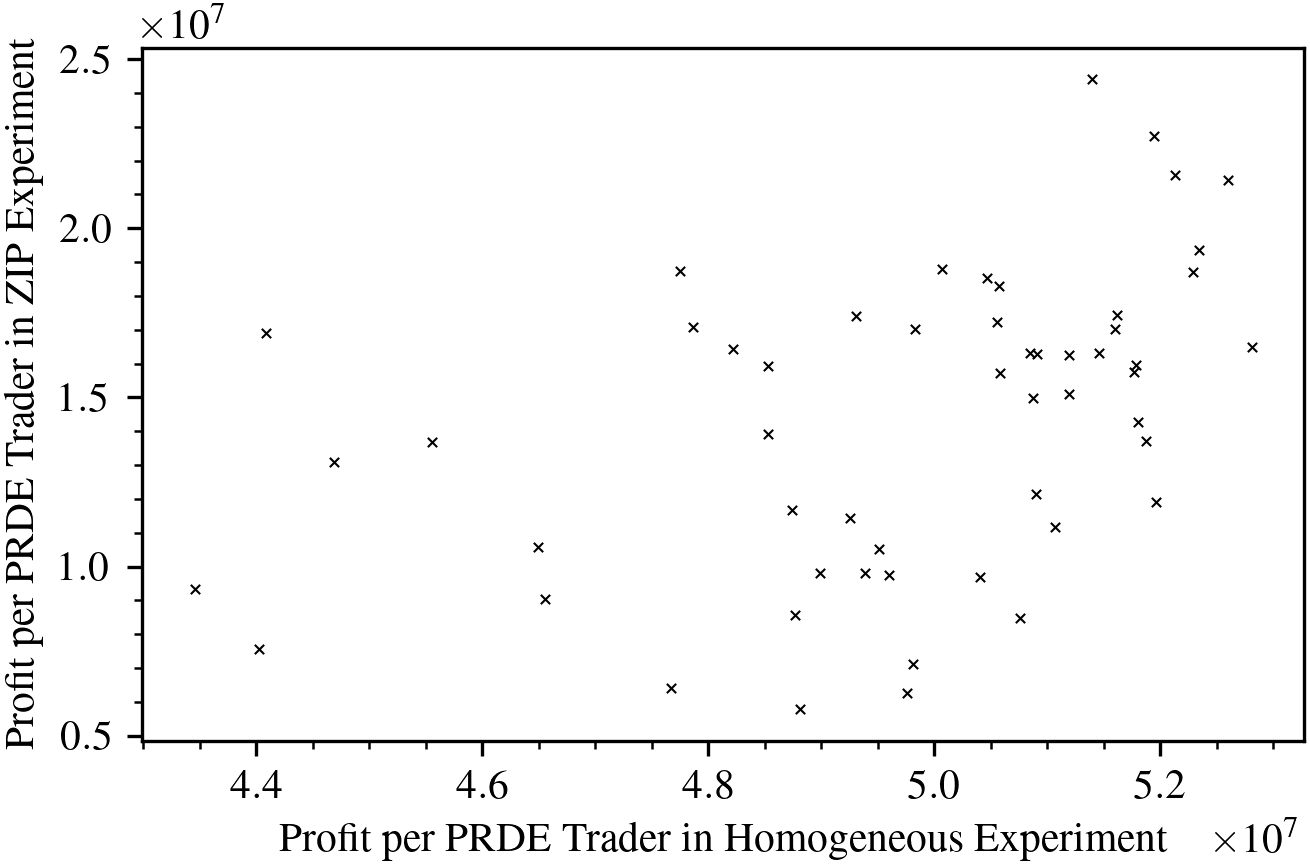
\includegraphics[width=\columnwidth]{homo_zip_scatter.png}}
    \caption{
        Relationship between the profitability per trader in the homogeneous PRDE experiments and the heterogeneous experiments.
        The horizontal axis is the mean profit per trader in a given homogeneous experiment for a specific combination of $F$ and $\mathrm{NP}$; the vertical axis is the mean profit per trader in a given heterogeneous experiment with the same $F$ and $\mathrm{NP}$.
        See text for further discussion.
    }
    \label{homo_zip_scatter}
\end{figure}

\section{Extending PRDE}

\subsection{PRZI with JADE}

In light of the problems with PRDE, this section introduces a new MI trader-agent: \textit{PRZI with JADE} (PRJADE), which replaces the DE algorithm in PRDE with a variation of JADE \cite{ZhangSanderson}.
JADE is a generational DE algorithm, and as such, a given trader $i$ maintains a population of candidate $s$-values for generation $g$ denoted $\mathcal{S}_{i,g}$.
Each $s$-value in $\mathcal{S}_{i,g}$, denoted $s_{i,g,1}, s_{i,g,2}, ..., s_{i,g,\mathrm{NP}}$, is evaluated in turn to produce a population of candidate $s$-values for the next generation $\mathcal{S}_{i,g+1}$.
Once strategy $s_{i,g,x}$ has been evaluated, three other distinct $s$-values are chosen:
\begin{itemize}
    \item $s^{p_i}_{i,g,\text{best}}$ is randomly chosen as one of the top $p_i\%$ of $s$-values in the population $\mathcal{S}_{i,g}$.
    \item $s_{i,g,r_1}$ is randomly chosen from the population $\mathcal{S}_{i,g}$ such that $s_{i,g,r_1}\ne s^{p_i}_{i,g,\text{best}}$.
    \item $\tilde{s}_{i,g,r_2}$ is randomly chosen from $\mathcal{S}_{i,g}\cup\mathcal{A}$ such that $\tilde{s}_{i,g,r_2}\ne s_{i,g,r_1}\ne s^{p_i}_{i,g,\text{best}}$, and where $\mathcal{A}$ is an `archive' set of $s$-values: those $s$-values that previously failed in the selection process.
\end{itemize}

Once these three values have been selected, a new candidate strategy $\hat{s}_{i,g,x}$ is constructed as follows:
\[
    \hat{s}_{i,g,x}\leftarrow s_{i,g,x}+F_{i,x}\left(s^{p_i}_{i,g,\text{best}} - s_{i,g,x}\right) + F_{i,x}\left(s_{i,g,r_1} - \tilde{s}_{i,g,r_2}\right)
\]
The fitness of $\hat{s}_{i,g,x}$ is evaluated, and if it performs better than $s_{i,g,x}$ then it is placed in index $x$ in $\mathcal{S}_{i,g+1}$. 
Otherwise, it is discarded, and the following strategy in the sequence $s_{i,g,x+1}$ is evaluated.

The main benefit that PRJADE provides over PRDE is that one does not need to initialise a PRJADE trader with a differential weight coefficient.
A given PRJADE trader $i$ generates a new $F_{i,x}$ for each new candidate strategy $\hat{s}_{i,g,x}$ in generation $g$ itself.
It does this according to a Cauchy distribution with location parameter $\mu_{F_i}$ and scale parameter $0.1$, which it then truncates to be two if $F_{i,x}>2$ or regenerated if $F_{i,x}<0$.
Sampling $F_{i,x}$ from the Cauchy distribution helps produce diverse differential weights centred around $\mu_{F_i}$, which can be considered a `best guess' at the optimal value for the differential weight.
$\mu_{F_i}$ is initialised to one at the start of the market session and then updated at the end of each generation using the following rule:
\[
    \mu_{F_i}\leftarrow (1-c_i)\mu_{F_i} + c_i\frac{\sum_{F\in \mathcal{F}_i} F^2}{\sum_{F\in\mathcal{F}_i} F}
\]
where $\mathcal{F}_i$ is a set of `successful' differential weights---those that yielded candidate strategies that increased profitability in generation $g$ for trader $i$.
Figure \ref{mu_F} shows how a PRJADE trader optimised its private $\mu_{F_i}$ value throughout a 100-day market simulation.

\begin{figure}[htbp]
    \centerline{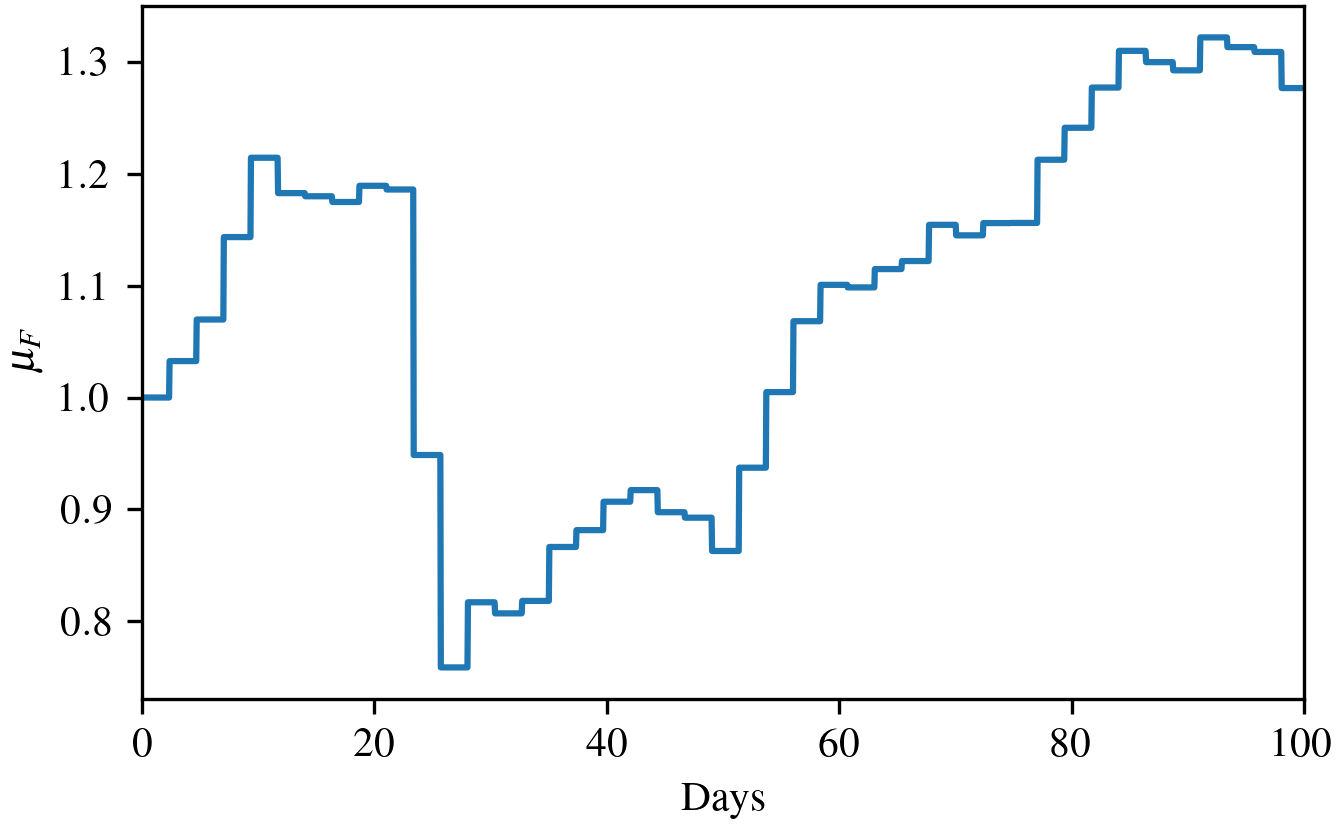
\includegraphics[width=\columnwidth]{mu_F_2.0.png}}
    \caption{
        Plot showing how the $\mu_{F_i}$ of a PRJADE trader can adapt through the market session.
        The horizontal axis is time, measured in days; the vertical axis is the $\mu_{F_i}$ value of a single PRJADE trader-agent.
        See text for further discussion.
    }
    \label{mu_F}
\end{figure}

Whilst PRJADE no longer requires the differential weight to be explicitly specified, it requires two new values: the rate of parameter adaption $c$ and the greediness of the mutation strategy $p$.
However, Zhang and Sanderson showed $c$ and $p$ to be insensitive to different problems in \cite{ZhangSanderson}, so they offer an advantage over the differential weight $F$, which I proved extremely sensitive to different market conditions in the previous sections.

\subsection{PRJADE vs PRDE}

In order to evaluate the performance of PRJADE, I took inspiration from IBM's balanced-group tests \cite{TesauroDas}.
I conducted a series of experiments in which an equal number of PRJADE and PRDE trader-agents competed against one another in the same market to identify which type of trader-agent would extract the most profit.
Since the performance of the PRDE agent had been particularly susceptible to varying the differential weight, I conducted three sets of experiments with $F=0$, $F=1$ and $F=2$ to determine whether PRJADE would be consistently `dominant'.
I initialised both the PRJADE and PRDE traders with $\mathrm{NP}=14$ in each experiment since the PRDE traders yielded reasonable profitability in all prior experiments with $\mathrm{NP}=14$.

I ran each trial with $N_T=20$ traders, split evenly between $N_B=10$ buyers and $N_S=10$ sellers.
The $N_B$ buyers and $N_S$ sellers comprised five PRDE traders and five PRJADE traders each.
Both groups were given evenly-spaced limit prices in the range $[60,140]$.
I ran each experiment for 100 simulated days.
In the simulation, after two traders engaged in a trade, they were rendered inactive until their stock was replenished, which occurred approximately every five simulated seconds.

The boxplots in Figure \ref{prjade_prde_boxplot} illustrate the results.
The PRJADE traders were consistently more profitable than the PRDE traders, regardless of the PRDE traders' differential weight.
Employing the Wilcoxon--Mann--Whitney U test and the Fligner--Pollicello robust rank-order distributional test proved a statistically significant improvement in the performance of the PRJADE traders across all three sets of experiments at the 1\% significance level.
Thus, I can be reasonably confident that PRJADE is `dominant' over PRDE over a range of values of $F$.
However, it is clear from the boxplots that the degree to which PRJADE is more profitable than PRDE depends on the differential weight of the PRDE traders.
As such, future work should explore more combinations of $F$ and $\mathrm{NP}$ to identify whether PRJADE is dominant definitively.

\begin{figure}[htbp]
    \centerline{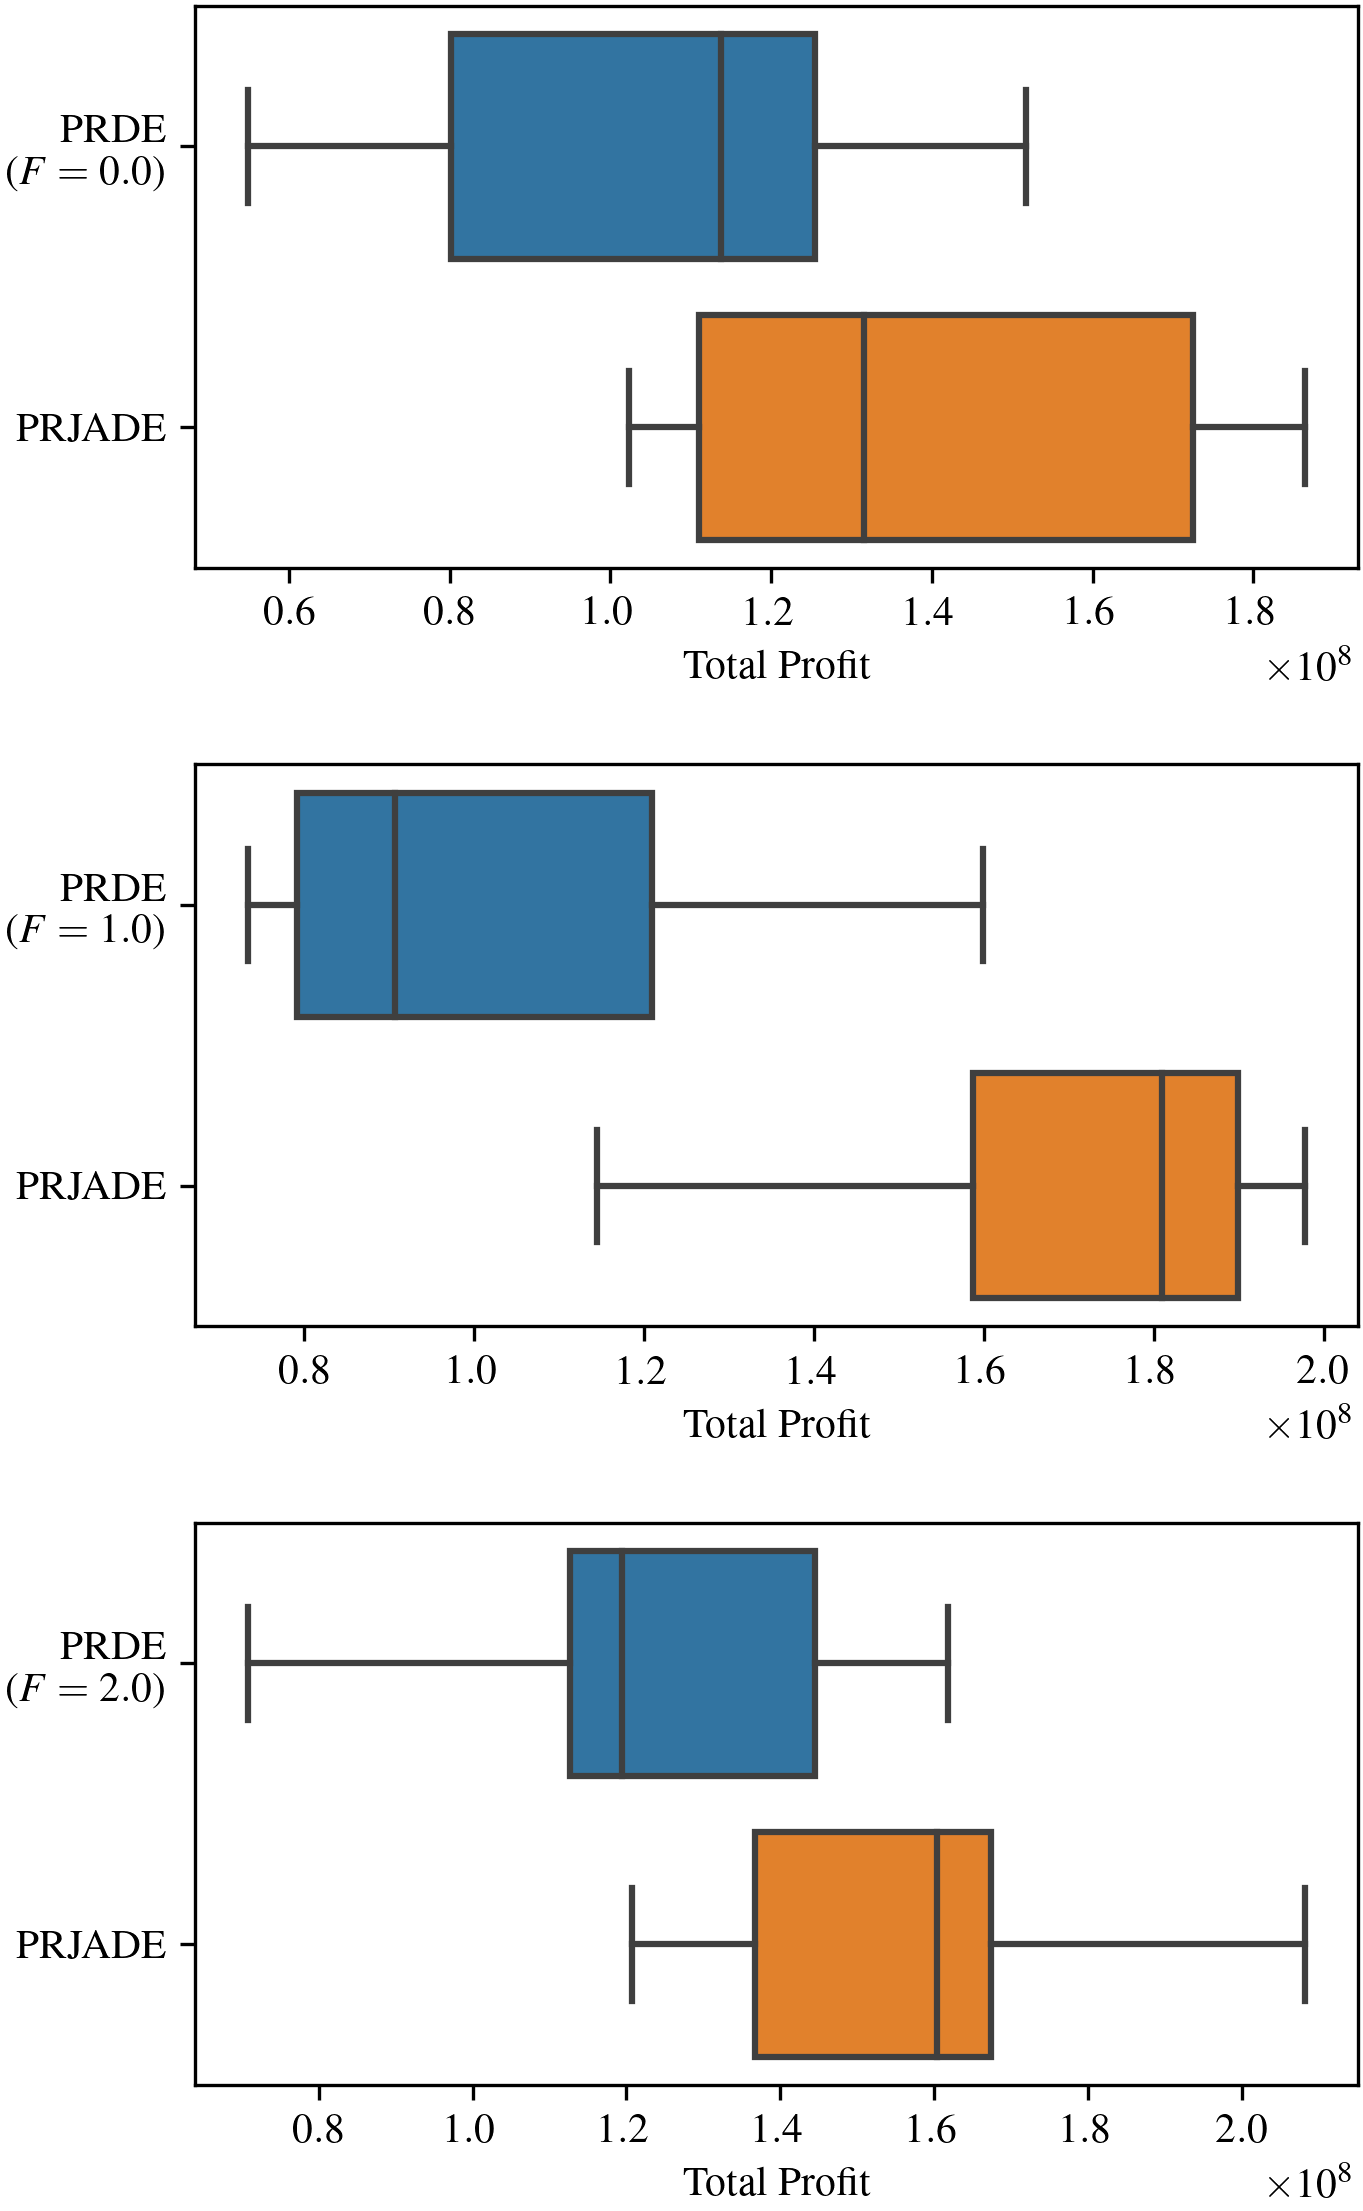
\includegraphics[width=\columnwidth]{prjade_prde_boxplot.png}}
    \caption{
        Three boxplots showing the performance of PRJADE against PRDE.
        In the top boxplot, all PRDE traders were configured with $F=0$; in the middle boxplot, all PRDE traders were configured with $F=1$; in the bottom boxplot, all PRDE traders were configured with $F=2$.
        In all experiments, both PRDE and PRJADE were configured with $\mathrm{NP}=14$.
        The horizontal axis is the combined profit extracted from the market by traders running the same algorithm (i.e. PRDE or PRJADE).
        See text for further discussion.
    }
    \label{prjade_prde_boxplot}
\end{figure}

\section{Conclusion}

This study has investigated the effects of the differential weight coefficient $F$ and the number in population $\mathrm{NP}$ on the dynamics of financial markets containing PRDE traders.
The first set of experiments focused on a market containing a homogeneous population of PRDE traders with perfect elasticity of supply and demand.
I identified a strong linear relationship between the `urgency' of the individual traders in these experiments and the total profit extracted from the market, which explained 72\% of the variance in profitability.
In this respect, the effect of $F$ on profitability could be primarily attributed to its impact on this urgency: a simple linear relationship with F could describe 77\% of the variance in urgency.
I found that the contribution of $\mathrm{NP}$ was more complex but could also be attributed to how it impacts the `urgency', though the relationship was nonlinear.

From the second set of experiments I conducted in heterogeneous markets with stepped supply and demand schedules, I identified that there appeared to be no correlation between the profitability of combinations of $F$ and $\mathrm{NP}$ in different market conditions.
The lack of association means there is unlikely to be an optimal combination that maximises profitability across multiple markets.
The optimal combination depends on the other traders' behaviour, the market's supply and demand schedules, or, most likely, a combination of both.
The lack of a market-independent optimal combination highlighted one of the primary limitations of the PRDE trader agent.
In that, despite the extreme sensitivity of its profitability to the parameters $F$ and $\mathrm{NP}$---especially in the heterogeneous experiments---the lack of an optimal combination means that one would almost require a priori information about the market to extract a near maximum amount of profit.

To address these limitations, I proposed the PRZI with JADE (PRJADE) trader-agent, an extension to PRDE that incorporates a self-adaptive mechanism for the differential weight parameter.
This extension enables PRJADE traders to adjust their differential weight based on market conditions, thus eliminating the problems associated with the extremely sensitive $F$ parameter.
The results indicate that PRJADE traders are more profitable than PRDE traders, even when the PRDE traders are initialised with different values of $F$.
However, further studies will be required to test the effectiveness of PRJADE against PRDE with different values of $\mathrm{NP}$, and more values of $F$, to confidently establish whether it consistently outperforms PRDE.
The results presented here also invite another line of future work: exploring the effect on the market's dynamics of the two new parameters in PRJADE, namely $p$ and $c$.
While Zhang and Sanderson proposed that these two parameters are insensitive to different problems in \cite{ZhangSanderson}, future research should confirm that this remains the case in PRJADE.

\bibliographystyle{IEEEtran}
\bibliography{refs}

\end{document}
